\section{匀变速直线运动习题精解}
\begin{calculate}
  1.一物体以某一速度冲上一光滑斜面,做匀变速直线运动,前$4s$ 的位移为$1.6m$ ,随后$4s$ 的位移为零,那么物体的加速度多大?

  a.物体的加速度大小为$0.1m/s^2$

  e.题目中所述运动情况如<:
  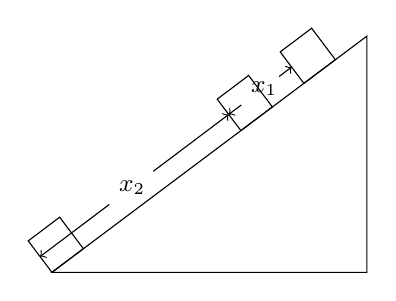
\begin{tikzpicture}
   \draw (0,0)--(4,0)--(4,3)-- cycle; 
   \draw[rotate=37] (0,0) rectangle (0.5,0.5);
   \draw[xshift=2.4cm ,yshift=1.8cm ,rotate=37] (0,0) rectangle (0.5,0.5);
   \draw[xshift=3.2cm ,yshift=2.4cm ,rotate=37] (0,0) rectangle (0.5,0.5);
   \draw[<-,rotate=37](0,0.25)--(1.1,0.25) node [anchor= south west] {\small $x_2$};
   \draw[->,rotate=37](1.8,0.25)--(3,0.25);
   \draw [<-,rotate=37] (3,0.25)--(3.2,0.25) node [anchor=south west]{\small $x_1$};
   \draw [->,rotate=37] (3.8,0.25)--(4,0.25);
  \end{tikzpicture}
  :>所示.由于随后的$4s$ 内位移为零,则可以判断出在这$4s$ 内先上升再下降,由对称性知向上运动$x_1$ 和向下运动 $x_1$的时间都是$2s$.所以记发生$x_2$ 位移的时间$t_2=4s$,发生$x_1$位移的时间 $t_1=2s$.
  \newline
  解法一:设初速度$v_0$,由匀变速直线运动位移与时间的关系\eqref{eq:x-t}式得
  $$x_2=v_0t_2+\cfrac{1}{2}at_2^2$$
  显然可以得到,物体到达最高点的速度为$0$ , 设从最低点到最高点所用时间为$t$ ,则$t=t_1+t_2=6s$,同样可以由\eqref{eq:x-t}式得
  $$x_1+x_2=v_0t+\cfrac{1}{2}at^2$$
  由上述二式联立解得
  \newline
  $$a=-0.1m/s^2 , v_0=0.6m/s$$

  ee.解法二:由平均速度公式\eqref{eq:v-average-half}可以得到前$4s$ 内的中间时刻的瞬时速度为 
  $$v=\cfrac{x_2}{t_2}=0.4m/s$$
  根据后 $2s$ 速度减到零,可得从第$2s$末到第$6s$末速度由$v=0.4m/s$ 减到零.所以可以由加速度定义\eqref{eq:acceleration}式得
  $$a=\cfrac{\Delta v}{\Delta t}=\cfrac{0-0.4m/s}{6s-2s}=-0.1m/s^2$$

  ee.解法三:将此运动视为反向的初速度为零的匀加速直线运动,由等分时间时位移的比例关系\eqref{eq:x-frac}可得,连续三段$T=2s$的位移比为$1:3:5$ ,所以可以得到
  $$x_1=\cfrac{1}{8}x_2=0.2m$$
 同时可以得到第二段时间内的位移为$0.6m$, 由相邻两段时间内的位移差公式\eqref{eq:Delta x} 得
  $$0.6m-0.2m=a^\prime (2s)^2$$
  解上式得
  $$a^\prime =\cfrac{0.6m-0.2m}{4s^2}=0.1m/s^2$$
  上式中加速度加撇的原因在于它是反向的匀加速直线运动,而正向的匀减速直线运动与它相差一个负号,即$a=-a'=-0.1m/s^2$.

  ee.解法四:考虑同第三种解法得到$x_1=0.2m$ ,仍然视为反向的匀加速直线运动,由匀变速直线运动公式\eqref{eq:x-t}关系得
  $$x_1=\cfrac{1}{2}a'T^2$$
  对上式简单运算得
  $$a'=\cfrac{2x_1}{T^2}=0.1m/s^2$$
  匀减速直线运动的加速度为$a=-a'=-0.1m/s^2$.

  ee.解法五:与解法二相同,由平均速度公式\eqref{eq:v-average-half}式得到中间时刻的瞬时速度$v=0.4m/s$,对于此后$4s$ 内物体将匀减速到速度为$0$,由平均速度公式\eqref{eq:average}可得后$4s$ 的位移为
  $$x=\cfrac{v+0}{2}\cdot t =0.8m$$
  由匀变速直线运动位移与速度的关系\eqref{eq:x-v}式得
  $$v^2-0^2=2ax$$
  解得
  $$a=-\cfrac{v^2}{2x}=-0.1m/s^2$$

  ee.同学们注意,在匀变速直线运动中往往会导致一题多解,但是归根结底都是相同的.只是按不同的思路考虑问题罢了,如果方法选择得当则题目会很轻松的得到解决,但是选择不当会增加不少的计算量.所以同学们在刚刚开始学习的时候最好能够尝试一题多解,练熟公式的同时找到解题的技巧.

  

\end{calculate}
\begin{calculate}
  2.一物体做匀加速直线运动,通过一段位移$\Delta x$ 所用的时间为$t_1$ ,紧接着通过下一段位移$\Delta x$ 所用时间为$t_2$ ,求物体运动的加速度.

  a.$\cfrac{2\Delta x(t_1-t_2)}{t_1t_2(t_1+t_2)}$

  e.物体通过第一段位移中间时刻的瞬时速度为$v_1=\frac{\Delta x}{t_1}$ ,通过第二段位移中间时刻的瞬时速度为$v_2=\frac{\Delta x}{t_2}$ ,由$v_1$ 变到$v_2$ 所需的时间显然为 $\Delta t=\frac{t_1+t_2}{2}$ ,由加速度定义\eqref{eq:acceleration} 式得
  $$a=\cfrac{v_2-v_1}{\Delta t}=\cfrac{2\Delta x(t_1-t_2)}{t_1t_2(t_1+t_2)}$$

  3.一质点运动的位移随时间变化的图象是一条抛线,方程为$x=-5t^2+40t$,则
  [1]求质点的初速度
  [2]求质点运动的加速度
  [3]求质点运动的最大位移
  [4]求质点速度为零时的时间

  a.见解析

  e.对比$x=-5t^2+40t$ 和 匀变速直线运动位移与时间的关系\eqref{eq:x-t} 可得

  ee.(1)质点运动的初速度为$v_0=40m/s$

  ee.(2)质点运动的加速度由对比可知$\frac{1}{2}a=-5m/s^2$,解得$a=-10m/s^2$.

  ee.(3)最大位移由匀变速直线运动\eqref{eq:x-v}式得
  $$0-v_0^2=2ax_m$$
  解得
  $$x_m=\cfrac{0-v_0^2}{2a}=80m$$
  
  ee.(4)由匀变速直线运动速度与时间的关系\eqref{eq:v-t}式得
  $$0=v_0+at$$
  解得
  $$t=-\cfrac{v_0}{a}=4s$$

  4.一辆汽车沿平直公路以速度$v_1$ 行驶了$\frac{2}{3}$ 的路程,接着又以速度$v_2=20km/h$ 行驶完其余 $\frac{1}{3}$ 的路程,如果汽车全程的平均速度为$28km/h$ ,那么汽车在前 $\frac{2}{3}$ 的路程内速度的大小为多少?

  a.$35km/h$

  e.由于汽车做单向直线运动则位移大小等于路程,设总位移为$x$ , 则前$\frac{2}{3}$ 所用的时间为 $t_1=\frac{2x}{3v_1}$ , 后 $\frac{1}{3}$ 所用时间为 $t_2=\frac{x}{3v_2} $ ,则总时间为 
  $$t=t_1+t_2=\cfrac{2x}{3v_1}+\cfrac{x}{3v_2}$$
  由平均速度公式 \eqref{eq:average} 得
  $$\overline{v}=\cfrac{x}{\frac{2x}{3v_1}+\frac{x}{3v_2}}$$
  上式约掉$x$ 然后经过简单计算得
  $$v_1=\cfrac{2\overline{v}v_2}{3v_2-\overline{v}}=35km/h$$
  注意:在这个题的计算中不要上来就化单位为国际单位,因为在计算中很明显的一点就是位移不知道,所以在计算中一定可以消去.这样一来,最后的结果应该就可以用与题目中相同的单位表达,并且一般会比较简洁,如果化单位的话,这个题目就走了弯路了.

  5.质点由A点静止出发沿直线 AB运动,行程的第一部分是加速度大小为 $a_1$ 的匀加速运动,接着做加速度大小为$a_2$ 的匀减速运动,到达B点时恰好速度减为零.若AB间总长度为$x$ , 则质点从A到B所用时间$t$ 为多少?

  a.$\sqrt{\cfrac{2x(a_1+a_2)}{a_1a_2}}$

  e.设第一阶段的末速度为$v$ , 则由题意据匀变速直线运动位移与速度关系\eqref{eq:x-v} 式可知:
  $$\cfrac{v^2}{2a_1}+\cfrac{v^2}{2a_2}=x$$
  由上式解得
  $$v=\sqrt{\cfrac{2a_1a_2x}{a_1+a_2}}$$
  而由匀变速直线运动位移计算基本关系\eqref{eq:displacement}式可得
  $$x=\cfrac{0+v}{2}t_1+\cfrac{v+0}{2}t_2=\cfrac{v}{2}t$$
  由此解得
  $$t=\sqrt{\cfrac{2(a_1+a_2)x}{a_1a_2}}$$

  6.美国``肯尼迪''号航空母舰上装有帮助飞机起飞的弹射系统.已知``F-15'' 型战斗机在跑道上加速时,产生的最大加速度为$5m/s^2$ ,起飞的最小速度是$50m/s^2$ ,弹射系统能够使飞机具有的最大速度为$30m/s$ ,则:
  [1]飞机起飞时在跑道上至少加速多长时间才能起飞?
  [2]航空母舰的跑道至少应该多长?

  a. (1)$4s$ (2)$160m$

  e.(1)飞机在跑道上运动的过程中,当有最大初速度、最大加速度时,起飞所需时间最短,据加速度的定义\eqref{eq:acceleration}或者匀变速直线运动速度与时间的关系\eqref{eq:v-t}得
  $$t=\cfrac{v-v_0}{a}=\cfrac{50-30}{5}s=4s$$
  则飞机起飞时在跑道上的加速时间至少为$4s$.

  ee.(2)由匀变速直线运动位移与时间的关系\eqref{eq:x-v} 式得
  $$x=\cfrac{v^2-v_0^2}{2a}=\cfrac{50^2-30^2}{2\times 5}m=160m$$
  即航空母舰的跑道至少为$160$.

  7.一质点做匀变速直线运动,初速度$v_0=2m/s$ , $4s$ 内位移为$20m$ ,求:
  [1]质点$4s$末的速度;
  [2]质点$2s$ 末的速度.

  a.(1)$8m/s$ (2) $5m/s$

  e.(1)利用平均速度公式\eqref{eq:average velocity}得$4s$ 内的平均速度为
  $$\overline{v}=\cfrac{x}{t}=\cfrac{v_0+v_4}{2}$$
  代入数据解得$4s$末的速度为
  $$v_4=8m/s$$

  ee.(2)由匀变速直线运动平均速度与位移中点的瞬时速度关系\eqref{eq:v-average-half}得$2s$ 末的速度为
  $$v_2=\cfrac{v_0+v_4}{2}=5m/s$$

  8.一个做匀加速直线运动的物体,在前$4s$ 内经过的位移为$24m$ ,在第$2$ 个$4s$ 内经过的位移是$60m$ ,求这个物体的加速度和初速度各是多少?

a.$2.25m/s^2$ $1.5m/s$

e.解法一:物体在前$4s$ 内的位移 
$$x_1=v_0t+\frac{1}{2}at^2$$
在第2个$4s$ 内的位移
$$x_2=v_0(2t)+\cfrac{1}{2}(2t)^2-(v_0t+\cfrac{1}{2}at^2)$$
将$x_1=24m$ ,$x_2=60m$ 代入上式,解得
$$a=2.25m/s^2,v_0=1.5m/s$$

ee.解法二:物体在$8s$ 内的平均速度等于中间时刻(第$4s$ 末)的瞬时速度,则
$$v_4=\cfrac{24+60}{8}m/s=10.5m/s$$
物体在前$4s$ 内的平均速度等于第$2s$ 末的瞬时速度
$$v_2=\cfrac{24}{4}m/s=6m/s$$
由加速度的定义可得
$$a=\cfrac{v_4-v_2}{\Delta t}=\cfrac{10.5-6}{2}m/s^2=2.25m/s^2$$
由匀变速直线运动速度与时间的关系得
$$v_2=v_0+at_2$$
解得
$$v_0=v_2-at_2=1.5m/s$$

ee.解法三:由等时相邻位移公式\eqref{eq:Delta x}得
$$a=\cfrac{\Delta x}{T^2}=\cfrac{60-24}{4^2}m/s^2=2.25m/s^2$$
同解法一$v_4=\frac{24+60}{8}m/s$,由匀变速直线运动速度与时间关系\eqref{eq:v-t} 式得
$$v_4=v_0+at_4$$
解得
$$v_0=1.5m/s$$

9.一辆汽车以$3m/s^2$ 的加速度开始启动的瞬间,另一辆以$6m/s$ 的速度做匀速直线运动的自行车恰好从汽车的旁边通过.
[1]汽车一定能追上自行车吗?若能追上,汽车经过多长时间追上?追上时汽车的瞬时速度多大?
[2]记汽车用2表示,自行车用1表示.在汽车追上自行车前,当$v_2<v_1$ 时,两者间的距离如何变化?当$v_2>v_1$时,两者间的距离如何变化?汽车追上自行车前多长时间与自行车相距最远?此时的距离是多大?

a.见解析

e.解法一:(1)因为汽车做加速运动,故汽车一定能追上自行车.汽车追上自行车时,两者位移相等,$x_2=x_1$,即
$$\cfrac{1}{2}at^2=v_1t$$
解得
$$t=\cfrac{2v_1}{a}=\cfrac{2\times6}{3}s=4s,v_2=at=3\times 4 m/s=12m/s$$

ee.(2)开始阶段,$v_2<v_1$ ,两者间的距离逐渐变大.后来$v_2>v_1$ ,两都间的距离又逐渐减小.所以汽车追上自行车前,当$v_2=v_1$ 时,两者距离最大.设经过时间$t_1$ ,汽车速度等于自行车速度,则
$$at_1=v_1$$
解得
$$t_1=2s$$
此时
$$x_1=v_1t_1=6\times2m=12m$$
$$x_2=\cfrac{1}{2}at_1^2=\cfrac{1}{2}\times3\times2^2m=6m$$
最大距离为
$$\Delta x=x_1-x_2=6m$$

ee.解法二:在第一个解法中偏重于物理情景的讨论,由于运动的情况可能要复杂的多,讨论就会变得复杂,所以这里介绍偏重数学计算的统一化讨论的方法.开始自行车在汽车前面,则分别写出二者在任意时刻$t$ 的位移分别为
$$x_1=v_1t , x_2=\cfrac{1}{2}at^2$$
由于自行车开始在汽车的前面,所以计算它们位移差的变化量 $\Delta x=x_1-x_2$ ,如果$\Delta x <0 $ 在$t>0$ 时成立,则汽车就可以追上自行车,反之则不能追上.
$$\Delta x=v_1t-\cfrac{1}{2}at^2$$
代入数值得$\Delta x $关于时间$t$ 的一元二次函数.如下
$$\Delta x=6t-\cfrac{3}{2}t^2, (t>0)$$
令$$\Delta x =0 $$ 得一元二次方程
$$6t-\cfrac{3}{2}t^2=0$$
上式容易解得$t_1=0 (\mbox{舍去}),t_2=4s$ ,所以经过$4s$ 汽车追上自行车.此时速度为
$$v=at_2=3\times 4 m/s=12m/s$$

ee.求函数$\Delta x=6t-\cfrac{3}{2}t^2, (t>0)$的极大值,则由二次函数的性质易得
$$t=-\cfrac{6}{2\times(-\frac{3}{2})}s=2s$$
时二车的相对距离$\Delta x$ 取最大,为
$$\Delta x_{max}=\cfrac{4\times(-\frac{3}{2})\times 0 - 6^2}{4\times(-\frac{3}{2})}=6m$$


10.车从静止开始以$1m/s^2$ 的加速度前进,在车开始运动的同时,车后$20m$ 处,某人骑自行车开始以$ 6m/s$ 的速度匀速追赶,能否追上?若不能追上,人与车的最小距离是多少?若能追上,什么时候追上?

a.不能 $2m$

e.开始运动时,车在前,人在后所以选择人的起点为坐标原点,以车和人运动的方向为正方向,则以2表示车,1表示人,则二者的位移分别为
$$x_1=6t$$
$$x_2=20+\cfrac{1}{2}\times 1\times t^2$$
任意时刻二者位移差为 $\Delta x = x_2-x_1$ 代入上述表达式得
$$\Delta x= 0.5t^2-6t +20 ,(t>0)$$
令$\Delta x=0$ 得一元二次方程,其判别式为
$$\Delta = (-6)^2-4\times 0.5 \times 20 =-4<0$$
所以无解,则人不能追上汽车.
由一元二次函数求极值可得
$$\Delta x_{min}=\cfrac{4\times 0.5 \times 20 - (-6)^2}{4\times 0.5}=2m$$

11.一滴雨滴从离地面 $20m$ 高的楼房屋檐自由下落,下落过程中用 $0.2s$ 的时间通过一个窗口,窗口的高度为 $2m$ , $g$ 取 $10m/s^2$ ,问:
[1]雨滴落地时的速度大小;
[2]雨滴落地前最后 $1s$ 内的位移大小;
[3]屋檐离地面的上边框有多高?

a.见解析

e.(1)由匀变速直线运动速度与位移的关系可得
$$v^2=2gh \Longrightarrow v=\sqrt{2gh}=20m/s$$

ee.(2)法一:雨滴在最后$1s$内的平均速度等于中间时刻的瞬时速度,中间时刻到最后共经历 $t_1=0.5s$ 所以有
$$v=\overline{v}+gt_1 \Longrightarrow \overline{v}=v-gt_1=15m/s$$
由位移等于平均速度乘以时间得
$$\Delta h=\overline{v}\Delta t_1 =15m$$

ee.法二:仍然采用平均速度的方法,先求出总时间,然后再求出最后$1s$的中间时刻,即
$$h=\frac{1}{2}gt^2 \Longrightarrow t=\sqrt{\frac{2h}{g}}=2s$$
所以最后$1s$ 的中间时刻即 $t=1.5s$ 时瞬时速度等于平均速度
$$\overline{v}=gt=15m/s$$
由位移等于平均速度乘以时间得
$$\Delta h=\overline{v}\Delta t_1 =15m$$

ee.法三:先求出总时间,然后再算出前 $1s$ 的时刻,并求出位移和总位移作差也可以得到最后 $1s$ 内的位移.即
$$h=\frac{1}{2}gt^2 \Longrightarrow t=\sqrt{\frac{2h}{g}}=2s$$
从下落开始到落地前$1s$经历的时间为$t_1=1s$ ,所以
$$h_1=\frac{1}{2}gt_1^2=5m$$
最后$1s$ 内的位移为
$$\Delta h=h-h_1=20m-5m=15m$$


ee.(3)在雨滴通过窗口的过程中,用时$0.2s$,所以它的中间时刻的瞬时速度等于平均速度为
$$\overline{v'}=\frac{2m}{0.2s}=10m/s$$
所以雨滴由屋檐到通过窗口的中间时刻所用时间为
$$t_0=\frac{\overline{v'}}{g}=1s$$
由此可得,雨滴由屋檐到窗口的时间为$t'=1s-0.1s=0.9s$ 所以屋檐离窗口上边框的高度为
$$h'=\frac{1}{2}gt'^2=4.05m$$

12.一辆值勤的警车停在公路边,当警员发现从他旁边以$10m/s$ 的速度匀速行驶的货车严重超载时,决定前去追赶,经过$5.5s$ 后警车发动起来,并以$2.5m/s^2$的加速度做匀加速运动,但警车的行驶速度必须控制在$90km/h$以内,问:
[1]警车在追赶货车的过程中,两车的最大距离是多少?
[2]警车发动后要经过多长时间 才能追上货车?

a.(1) 75m \qquad (2) 12s

e.(1)以警车发动起来作为计时起点,首先将警车的最大速度切换成国际单位 $90km/h=25m/s$ ,则警车的加速过程的持续时间$t_m$ 为
$$v_m=at_m \Longrightarrow t_m=\frac{v_m}{a}=10s$$
写出$0\sim 10s$ 内两车的距离为
$$\Delta x=55+10t -\frac{5}{4}t^2$$
整理成标准一元二次方程
$$\Delta x =-\frac{5}{4}t^2+10t+55 \quad (m)$$
由二次函数的知识,易得在$0\sim 10s$内 $t=4s$ 时距离最大,为
$$\Delta x_{max}=75m$$

ee.注意,在警车追赶货车的过程中,要分两步考虑,在$0\sim 10s$ 内,两车的距离关系才是上述的一元二次函数,但是这个过程不一定就追上,所以不能直接使用$\Delta x=0$ 来计算出时间,这就导致错误了!! 最好的方法就是画出这段时间内的函数图象,然后得出能否在 $10s$ 内追上的明确结论.容易得到 $t=10s$ 时
$$\Delta x'=-\frac{5}{4}\times 10^2 +100 +55m =30m$$
于是加速过程结束时,警车没有追上货车,所以还要匀速追一段时间$t'$ 所以
$$t'=\cfrac{\Delta x'}{v_2-v_1}=2s$$
则警车追赶货车共用时间为
$$t=t_m+t'=12s$$

13.某人骑自行车以$v_1=4m/s$ 的速度前进,某时刻在他前面$x_0=7m$ 处有以$v_1=10m/s$ 的速度同向行驶的汽车开始关闭发动机减速前进,而以$a=-2m/s^2$ 的加速度匀减速前进,求:
[1]此人追上汽车之前落后于汽车的最大距离?
[2]此人需要多长时间才能追上汽车?

a.(1) 16m \qquad (2) 8s

e.(1)此问题出现了刹车,所以先求出刹车时间$t_s$
$$0=v_0+at_s \Longrightarrow t_s=-\frac{v_0}{a}=5s$$
容易写出$0\sim 5s$ 内两车的距离为
$$\Delta x = (7+10t-t^2)-4t $$
化成标准形式
$$\Delta x=-t^2+6t+7 \quad (m)$$
由一元二次方程得$t=3s$ 时,二者距离最大为
$$\Delta x_{max}=16m$$

ee.(2)注意,只有在$0\sim 5s$ 内二者的距离才按上述方程变化,但是不能保证$5s$ 内一定能追上,这需要单独判断.易得$t=5s$ 时,二者距离为
$$\Delta x'=-5^2+6\times 5 +7 m =12m$$
在$5s$时,人还没有追上汽车,而这时汽车已经停止运动,所以剩下的这$12m$ 人需要匀速追击,其所需时间$t'$ 为
$$t'=\frac{\Delta x'}{v_1}=3s$$
所以人追车的总时间为
$$t=t_s+t'=8s$$


14.甲、乙两车从\CJKunderwave{同一地点}出发,同向运动,其$v-t$ 图象如
<:
\begin{tikzpicture}
  \draw[->] (0,0)--(0,2.2) node [anchor=west]{\tiny $v/m\cdot s^{-1}$}; 
  \draw[->] (0,0)--(2.5,0) node [anchor= north]{\tiny $t/s$};
  \draw (0.5,0) node [anchor=north] {\tiny $2$};
  \draw (1,0) node [anchor=north] {\tiny $4$};
  \draw (1.5,0) node [anchor=north] {\tiny $6$};
  \draw (2,0) node [anchor=north] {\tiny $8$};
  \draw (0,0.3) node [anchor=east]{\tiny $1$};
  \draw (0,0.6) node [anchor=east]{\tiny $2$};
  \draw (0,0.9) node [anchor=east]{\tiny $3$};
  \draw (0,1.2) node [anchor=east]{\tiny $4$};
  \draw (0,1.5) node [anchor=east]{\tiny $5$};
  \draw (0,0)--(1,0.9)--(1.5,1.35);
  \draw (0.5,0)--(1,0.9)--(1.5,1.8);
  \draw[dotted] (1,0.9)--(0,0.9);
  \draw[dotted] (1,0.9)--(1,0);
  \draw[dotted] (1.5,0)--(1.5,1.85);
  \draw (1.5,1.35) node [anchor=north] {\tiny 甲};
  \draw (1.5,1.85) node [anchor=east] {\tiny 乙};
\end{tikzpicture}
:>所示.试计算:
[1]甲乙两车的加速度各为多大?
[2]两车相遇前的最大距离为多少?
[3]从乙车开始运动起经过多长时间后两车相遇?(计算结果保留$2$位小数)

a.(1) $a_{\mbox{\tiny 甲}}=\frac{3}{4}m/s^2$ \qquad $a_{\mbox{\tiny 乙}}=\frac{3}{2}m/s^2$ \qquad (2) $3m$ \qquad (3) $4.83s$

e.(1)由加速度的定义根据图象易得,计算从略.

ee.(2)如<:
\begin{tikzpicture}
  \draw[->] (0,0)--(0,2.2) node [anchor=west]{\tiny $v/m\cdot s^{-1}$}; 
  \draw[->] (0,0)--(2.5,0) node [anchor= north]{\tiny $t/s$};
  \draw (0.5,0) node [anchor=north] {\tiny $2$};
  \draw (1,0) node [anchor=north] {\tiny $4$};
  \draw (1.5,0) node [anchor=north] {\tiny $6$};
  \draw (2,0) node [anchor=north] {\tiny $8$};
  \draw (0,0.3) node [anchor=east]{\tiny $1$};
  \draw (0,0.6) node [anchor=east]{\tiny $2$};
  \draw (0,0.9) node [anchor=east]{\tiny $3$};
  \draw (0,1.2) node [anchor=east]{\tiny $4$};
  \draw (0,1.5) node [anchor=east]{\tiny $5$};
  \draw (0,0)--(1,0.9)--(1.5,1.35);
  \draw (0.5,0)--(1,0.9)--(1.5,1.8);
  \draw[dotted] (1,0.9)--(0,0.9);
  \draw[dotted] (1,0.9)--(1,0);
  \draw[dotted] (1.5,0)--(1.5,1.85);
  \draw (1.5,1.35) node [anchor=north] {\tiny 甲};
  \draw (1.5,1.85) node [anchor=east] {\tiny 乙};
  \draw [pattern=north west lines] (0,0)--(1,0.9)--(0.5,0);
\end{tikzpicture}
:>所示,由于$v-t$图象与$t$轴所围图形的面积表示位移,同时两车又是从\CJKunderwave{同一位置}开始运动,则开始时甲比乙快,所以甲比乙领先,于是两车位移差就是它们的距离,对应图中所示阴影面积就是两车的最大距离.即
$$\Delta x_{max}=\frac{1}{2}\times 2\times 3 m=3m$$

ee.(3)两车的距离随时间变化的规律容易得到,即
$$\Delta x=\frac{1}{2}a_{\mbox{\tiny 甲}}(t+2)^2-\frac{1}{2}a_{\mbox{\tiny 乙}}t^2$$
令$\Delta x =0$ 得
$$(\frac{t+2}{t})^2=\cfrac{a_{\mbox{\tiny 乙}}}{\mbox{\tiny 甲}}=2$$
解得$t=2(\sqrt{2}+1)s$ 由于题目中要求保留$2$位小数,所以取为
$$t=2(\sqrt{2}+1)s\approx 4.83s$$
{\bf 注意}使用速度时间图象法可以确定两车的最大距离,但是应该特别注意这点在{\bf 两车初始时刻位于同一位置}时才可行,如果\CJKunderwave{不是同一位置}则还是应该列出具体方程来讨论它们之间的距离随时间的变化才行,因此这属于一种特殊情况.

15.屋檐第隔相同的时间间隔滴下一滴水,当第$5$滴正欲下时,第$1$滴刚好到地面,而第$3$滴与第$2$滴分别位于高为 $1$米的窗子的上、下沿,如
<:
\begin{tikzpicture}
  \filldraw [color=black] (0,0) node [anchor=east] {\small 1} circle [radius=2pt]; 
  \filldraw [color=black] (0,1.4) node [anchor=east] {\small 2} circle [radius=2pt]; 
  \filldraw [color=black] (0,2.4) node [anchor=east] {\small 3} circle [radius=2pt]; 
  \filldraw [color=black] (0,3) node [anchor=east] {\small 4} circle [radius=2pt]; 
  \filldraw [color=black] (0,3.2) node [anchor=east] {\small 5} circle [radius=2pt]; 
  \draw [pattern=north west lines] (-0.5,-7pt)--(-0.5,-2.5pt)--(0.5,-2.5pt)--(0.5,-7pt);
\end{tikzpicture}
:>
所示不计空气阻力.求此屋檐离地面的高度及滴水的时间间隔.($g$取$10m/s^2$)

a.屋檐离地面高度为$3.2m$ ,滴水的时间间隔为$0.2s$

e.记第3滴和第2滴水滴的高度差为$\Delta h$ ,设滴水的时间间隔为$T$ ,则
法一:计算出第5滴水到第3滴水的距离和第5滴水到第2滴水的距离,二者的差就是窗户的高度了.即
$$\Delta h=\frac{1}{2}g(3T)^2-\frac{1}{2}g(2T)^2$$
解得
$$T=\sqrt{\frac{2\Delta h}{5g}}=0.2s$$
则屋檐离地面的高度$h$为
$$h=\frac{1}{2}g(4T)^2=3.2m$$

ee.法二:此题也可以借助于平均速度等于中间时刻的瞬时速度来解.由$\Delta h$ 可以计算出第2滴水滴和第3滴水滴之间的平均速度,此速度等于中间时刻$2.5T$ 的瞬时速度,即
$$\frac{\Delta h}{T}=g\cdot \frac{5}{2}T$$
解得
$$T=\sqrt{\frac{2\Delta h}{5g}}=0.2s$$
则屋檐离地面的高度$h$为
$$h=\frac{1}{2}g(4T)^2=3.2m$$

ee.法三:此题也可以借助初速度为零的比例式来求解.这四段距离之比为
$$1:3:5:7$$
所以第2滴水滴和第3滴水滴的距离占5份,而总共是$1+3+5+7=16$ 份,所以总的高度为
$$h=\frac{16}{5}\times 1m=3.2m$$
第5滴水滴到第4滴水滴的时间就是时间间隔$T$,即
$$\frac{1}{5}\Delta h=\frac{1}{2}gT^2$$
解得
$$T=\sqrt{\frac{2\Delta h}{5g}}=0.2s$$

16.A、B两辆汽车在笔直的公路上同向行驶.当B车在A车前$84m$处时,B 车的速度为$4m/s$,且正以$2m/s^2$的加速度做匀加速直线运动;经过一段时间后,B车的加速度突然变成零.A车一直以$20m/s$ 的速做匀速运动.经过$12s$后两车相遇.问B车加速行驶的时间是多少?

a.B车加速行驶的时间是$6s$

e.$12s$后A车的位移为
$$x_A=v_At_m=240m$$
则由于两车开始相距$84m$,所以B车的位移为
$$x_B=240m-84m=156m$$
设B车加速行驶的时间为$t$,则
$$x_B=v_{B0}t+\frac{1}{2}at^2+(v_{B0}+at)(t_m-t)$$
代入数值得关于时间的一元二次方程为
$$t^2-24t+108=0$$
采用十字相乘法得
$$(t-6)(t-18)=0$$
由于$t<12s$所以解得B车加速行驶的时间为
$$t=6s$$

16.利用水滴下落可以测出重力加速度$g$,调节水龙头,让水一滴一滴地流出,在水龙头的正下方放一个盘子,调整盘子的高度,使一个水滴碰到盘子时,恰好有一滴从水龙头开始下落,而空中还有一个正在下落的水滴,测出水龙头到盘子的距离为$h$,再从第一滴离开水龙头开始计时,到第$N$滴落到盘中,测出共用时间为$t$,求
[1]当第一滴落到盘子时,第二滴水滴离开水龙头的距离为多少?
[2]两滴水间的时间间隔是多少?
[3]重力加速度$g$是多大?

a.见解析

e.(1)利用初速度为零的匀变速直线运动的比例关系可得,第二滴水离开水龙头的距离与第一滴水离开水龙头的距离之比为$1:4$,所以第二滴水滴离开水龙头的距离为$\frac{h}{4}$

ee.(2)如<:
\begin{tikzpicture}
  \draw [pattern=north west lines] (-1,-0.2)--(-1,0)--(1,0)--(1,-0.2);
  \draw (-0.6,3.2)--(-0.6,2.9)--(-0.4,2.9)--(-0.4,3.2);
  \filldraw [color=black] (-0.5,2.8) circle [radius=1mm];
  \draw (-0.5,2.8) node [anchor=west] {\small $2$};
  \filldraw [color=black] (-0.5,2.1) circle [radius=1mm];
  \draw (-0.5,2.1) node [anchor=west] {\small $1$};
  \draw (0.6,3.2)--(0.6,2.9)--(0.4,2.9)--(0.4,3.2);
  \filldraw [color=black] (0.5,2.8) circle [radius=1mm];
  \draw (0.5,2.8) node [anchor=west] {\small $3$};
  \filldraw [color=black] (0.5,2.1) circle [radius=1mm];
  \draw (0.5,2.1) node [anchor=west] {\small $2$};
  \filldraw[color=black] (0.5,0.1) circle [radius=0.1];
  \draw (0.5,0.1) node [anchor=west] {\small $1$};
\end{tikzpicture}
:>所示,设两滴水滴下落间隔为$T$,其中第一滴下落到盘中所需时间为$2T$,再过$T$第二滴水下落到盘中,而之前第二滴水的位置已经被第三滴水占据,所以再过$T$第三滴水落到盘中,因此以后每隔一个$T$就有一滴水落到盘中,则第一滴水之后一共有$N-1$滴水滴,所以总时间为
$$2T+(N-1)T=t$$
解得,两滴水间的时间间隔是
$$\frac{t}{N+1}$$

ee.上面的这个情况还可以推广,如果空中有$m$个水滴,则第一滴水下落到盘中需要$m+1$个$T$,之后每个$T$就有一个水滴落入盘中,所以总时间为$(m+1)T+(N-1)T=(N+m)T$,因此$T$为
$$T=\frac{t}{N+m}$$

ee.(3)第一个$T$内水滴下落的距离已经由第(1)问求出,由自由落体位移与时间的关系得
$$\frac{h}{4}=\frac{1}{2}gT^2$$
解得
$$g=\frac{h}{2T^2}$$
将(2)中计算的时间间隔代入上式得
$$g=\frac{h(N+1)^2}{2t^2}$$

\end{calculate}

